\documentclass[
    article,
	% -- opções da classe memoir --
	12pt,				% tamanho da fonte
	openright,			% capítulos começam em pág ímpar (insere página vazia caso preciso)
	oneside,			% para impressão em verso e anverso. Oposto a oneside
	a4paper,			% tamanho do papel.
	sumario=abnt-6027-2012,
	% -- opções da classe abntex2 --
	chapter=TITLE,		% títulos de capítulos convertidos em letras maiúsculas
	section=TITLE,		% títulos de seções convertidos em letras maiúsculas
	%subsection=TITLE,	% títulos de subseções convertidos em letras maiúsculas
	%subsubsection=TITLE,% títulos de subsubseções convertidos em letras maiúsculas
	% -- opções do pacote babel --
	%english,			% idioma adicional para hifenização
	%french,				% idioma adicional para hifenização
	%spanish,			% idioma adicional para hifenização
	brazil				% o último idioma é o principal do documento
	]{abntex2}


% --- 
% CONFIGURAÇÕES DE PACOTES
% --- 
% ---
% Pacotes básicos 
% ---
\usepackage{lmodern}			% Usa a fonte Latin Modern			
\usepackage[T1]{fontenc}		% Selecao de codigos de fonte.
\usepackage[utf8]{inputenc}		% Codificacao do documento (conversão automática dos acentos)
\usepackage{lastpage}			% Usado pela Ficha catalográfica
\usepackage{indentfirst}		% Indenta o primeiro parágrafo de cada seção.
\usepackage{color}				% Controle das cores
\usepackage{graphicx}			% Inclusão de gráficos
\usepackage{microtype} 			% para melhorias de justificação
\usepackage{ufc-abntex2}
\usepackage{enumitem}
\usepackage{amsmath}
\usepackage{booktabs}
\usepackage{multirow}
\usepackage{titlesec}


%My Packages
\usepackage{threeparttable}
\usepackage{wasysym}

\renewcommand{\apendicesname}{AP\^ENDICES}


%Deixando o Caption centralizado mesmo com quebra de linha 
\usepackage[labelfont=bf, justification=centering]{caption}

%formatação do Sumário
\usepackage{etoolbox}                               
% Usado para alterar a fonte da Section no Sumário
\usepackage[nogroupskip,nonumberlist,acronym]{glossaries}                %
% ---
		
% ---
% Pacotes adicionais, usados apenas no âmbito do Modelo Canônico do abnteX2
% ---
\usepackage{lipsum}				% para geração de dummy text
% ---


% ---
% Pacotes de citações
% ---
%\usepackage[brazilian,hyperpageref]{backref}	 % Paginas com as citações na 
%bibl
%\usepackage[alf]{abntex2cite}	% Citações padrão ABNT


\usepackage[alf, abnt-emphasize=bf, bibjustif, recuo=0cm, abnt-etal-cite=2, abnt-etal-list=0]{abntex2cite} 

% Ambiente para alineas e e subalineas (incisos) com ponto
\newlist{alineascomponto}{itemize}{2}
\setlist[alineascomponto,1]{label={$\bullet$},topsep=0pt,itemsep=0pt,leftmargin=\parindent+\labelwidth-\labelsep}%
\setlist[alineascomponto,2]{label={--},topsep=0pt,itemsep=0pt,leftmargin=*}
\newlist{subalineascomponto}{enumerate}{1}
\setlist[subalineascomponto,1]{label={$\circ$},topsep=0pt,itemsep=0pt,leftmargin=*}%
% ---

% Ambiente para alineas e e subalineas (incisos) com numeros
\newlist{alineascomnumero}{enumerate}{2}
\setlist[alineascomnumero,1]{label={$\arabic*$.},topsep=0pt,itemsep=0pt,leftmargin=\parindent+\labelwidth-\labelsep}%
\setlist[alineascomnumero,2]{label={--},topsep=0pt,itemsep=0pt,leftmargin=*}
\newlist{subalineascomnumero}{enumerate}{1}
\setlist[subalineascomnumero,1]{label={$\arabic*$.},topsep=0pt,itemsep=0pt,leftmargin=*}%
% ---

% ---
% Configurações do pacote backref
% Usado sem a opção hyperpageref de backref
%\renewcommand{\backrefpagesname}{Citado na(s) página(s):~}
% Texto padrão antes do número das páginas
%\renewcommand{\backref}{}
% Define os textos da citação
%\renewcommand*{\backrefalt}[4]{
%	\ifcase #1 %
%		Nenhuma citação no texto.%
%	\or
%		Citado na página #2.%
%	\else
%		Citado #1 vezes nas páginas #2.%
%	\fi}%
% ---

% ---
% Configurações de aparência do PDF final

% alterando o aspecto da cor azul
\definecolor{blue}{RGB}{41,5,195}

% informações do PDF
\makeatletter
\hypersetup{
     	%pagebackref=true,
		pdftitle={\@title}, 
		pdfauthor={\@author},
    	pdfsubject={\imprimirpreambulo},
	    pdfcreator={LaTeX with abnTeX2},
		pdfkeywords={abnt}{latex}{abntex}{abntex2}{trabalho acadêmico}, 
		colorlinks=false,       		% false: boxed links; true: coloredlinks
    	linkcolor=blue,          	% color of internal links
    	citecolor=blue,        		% color of links to bibliography
    	filecolor=magenta,      		% color of file links
		urlcolor=blue,
		bookmarksdepth=4
}
\makeatother
% --- 

\makeatletter
\def\@biblabel#1{}
\renewenvironment{thebibliography}[1]
     {\section*{\refname}%
      \@mkboth{\MakeUppercase\refname}{\MakeUppercase\refname}%
      \list{\@biblabel{\@arabic\c@enumiv}}%
           {\settowidth\labelwidth{\@biblabel{#1}}%
            \leftmargin\labelwidth
            %\advance\leftmargin\labelsep
            \@openbib@code
            \usecounter{enumiv}%
            \let\p@enumiv\@empty
            \renewcommand\theenumiv{\@arabic\c@enumiv}}%
      \sloppy
      \clubpenalty4000
      \@clubpenalty \clubpenalty
      \widowpenalty4000%
      \sfcode`\.\@m}
     {\def\@noitemerr
       {\@latex@warning{Empty `thebibliography' environment}}%
      \endlist}
\makeatother


% --- 
% Espaçamentos entre linhas e parágrafos 
% --- 

% O tamanho do parágrafo é dado por:
\setlength{\parindent}{1.3cm}

% Controle do espaçamento entre um parágrafo e outro:
\setlength{\parskip}{0.2cm}  % tente também \onelineskip

% ---
% compila o indice
% ---
\makeindex
% ---



\usepackage{hyperref}% http://ctan.org/pkg/hyperref
\hypersetup{%
  colorlinks = false,
  linkcolor  = black,
  pdftitle={Ambiente Virtual de Aprendizagem para Auxiliar no Processo de Ensino e Aprendizagem de Matemática}
}

\addto\captionsbrazil{
	%% ajusta nomes padroes do babel
	\renewcommand{\bibname}{REFER\^ENCIAS}
	\renewcommand{\indexname}{\’Indice}
	\renewcommand{\listfigurename}{Lista de ilustra\c{c}\~{o}es}
	\renewcommand{\listtablename}{Lista de tabelas}
	%% ajusta nomes usados com a macro \autoref
	\renewcommand{\chapterautorefname}{Ap\^endice}
	\renewcommand{\pageautorefname}{P\’agina}
	\renewcommand{\sectionautorefname}{Se{\c c}\~ao}
	\renewcommand{\subsectionautorefname}{Se{\c c}\~ao}
	\renewcommand{\subsubsectionautorefname}{Se{\c c}\~ao}
}


\newcommand\fnote[1]{\captionsetup{font=small}\caption*{#1}}

% Informações de dados para CAPA e FOLHA DE ROSTO
\titulo{Ambiente Virtual de Aprendizagem para Auxiliar no Processo de Ensino e Aprendizagem de Matemática}
\autor{Marciano Machado Saraiva}
\local{Quixadá}
\data{Julho, 2016}
\orientador{Prof. Me. Samy Soares Passos de Sá}
%\coorientador{Nome Coorientador}

% Escolher curso: Redes de Computadores (rc), Eng.Software (es), Ciências da Computação (cc) ou Sist.Informação (si)
%\instituicao{%
Universidade Federal do Ceará \par
Campus Quixadá \par
Curso de Redes de Computadores
}
\tipotrabalho{Trabalho de Conclusão de Curso (Monografia)}
\preambulo{Monografia apresentada ao Curso de Redes de Computadores do Campus Quixadá da Universidade Federal do Ceará, como requisito parcial para obtenção do Título de Tecnólogo em Redes de Computadores.}

\instituicao{%
Universidade Federal do Ceará \par
Campus Quixadá \par
Curso de Sistemas de Informação
}
\tipotrabalho{Trabalho de Conclusão de Curso (Monografia)}
\preambulo{Monografia apresentada ao Curso de Sistemas de Informação do Campus Quixadá da Universidade Federal do Ceará, como requisito parcial para obtenção do Título de Bacharel em Sistemas de Informação.}

%\instituicao{%
Universidade Federal do Ceará \par
Campus Quixadá \par
Curso de Engenharia de Software
}
\tipotrabalho{Trabalho de Conclusão de Curso (Monografia)}
\preambulo{Monografia apresentada ao Curso de Engenharia de Software do Campus Quixadá da Universidade Federal do Ceará, como requisito parcial para obtenção do Título de Bacharel em Engenharia de Software.}

%\instituicao{%
Universidade Federal do Ceará \par
Campus Quixadá \par
Curso de Ciências da Computação
}
\tipotrabalho{Trabalho de Conclusão de Curso (Monografia)}
\preambulo{Monografia apresentada ao Curso de Ciências da Computação do Campus Quixadá da Universidade Federal do Ceará, como requisito parcial para obtenção do Título de Bacharel em Ciências da Computação.}


%%criar um novo estilo de cabeçalhos e rodapés
\makepagestyle{header_style}
  %%cabeçalhos
  \makeoddhead{header_style} %%pagina ímpar ou com oneside
     {}
     {}
     {\thepage} 


\begin{document}
\frenchspacing 

%Formatação de título de seções
\titleformat{\section}
{\normalfont\normalsize\bfseries}{\thesection}{1em}{}
\titleformat{\subsection}
{\normalfont\normalsize\bfseries}{\thesubsection}{1em}{}
\titleformat{\subsubsection}
{\normalfont\normalsize\bfseries}{\thesubsubsection}{1em}{}

% ----------------------------------------------------------
% ELEMENTOS PRÉ-TEXTUAIS
% ----------------------------------------------------------
% \pretextual
% Capa
\imprimircapa

%----------- Apenas TCC 2
% Folha de rosto (* indica que haverá a ficha bibliográfica)
%\imprimirfolhaderosto

% Ficha Bibliográfica
%% ---
% Inserir a ficha bibliografica
% ---

% Isto é um exemplo de Ficha Catalográfica, ou ``Dados internacionais de
% catalogação-na-publicação''. Você pode utilizar este modelo como referência. 
% Porém, provavelmente a biblioteca da sua universidade lhe fornecerá um PDF
% com a ficha catalográfica definitiva após a defesa do trabalho. Quando estiver
% com o documento, salve-o como PDF no diretório do seu projeto e substitua todo
% o conteúdo de implementação deste arquivo pelo comando abaixo:
%
% \begin{fichacatalografica}
%     \includepdf{fig_ficha_catalografica.pdf}
% \end{fichacatalografica}
\begin{fichacatalografica}
	\vspace*{\fill}					% Posição vertical
	\hrule							% Linha horizontal
	\begin{center}					% Minipage Centralizado
	\begin{minipage}[c]{12.5cm}		% Largura
	
	\imprimirautor
	
	\hspace{0.5cm} \imprimirtitulo  / \imprimirautor. --
	\imprimirlocal, \imprimirdata-
	
	\hspace{0.5cm} \pageref{LastPage} p. : il. (algumas color.) ; 30 cm.\\
	
	\hspace{0.5cm} \imprimirorientadorRotulo~\imprimirorientador\\
	
	\hspace{0.5cm}
	\parbox[t]{\textwidth}{\imprimirtipotrabalho~--~\imprimirinstituicao,
	\imprimirdata.}\\
	
	\hspace{0.5cm}
		1. Palavra-chave1.
		2. Palavra-chave2.
		I. Orientador.
		II. Universidade xxx.
		III. Faculdade de xxx.
		IV. Título\\ 			
	
	\hspace{8.75cm} CDU 02:141:005.7\\
	
	\end{minipage}
	\end{center}
	\hrule
\end{fichacatalografica}
% ---

% Errata
%% ---
% Inserir errata
% ---
\begin{errata}
Elemento opcional da NORMA. Exemplo:

\vspace{\onelineskip}

FERRIGNO, C. R. A. \textbf{Tratamento de neoplasias ósseas apendiculares com
reimplantação de enxerto ósseo autólogo autoclavado associado ao plasma
rico em plaquetas}: estudo crítico na cirurgia de preservação de membro em
cães. 2011. 128 f. Tese (Livre-Docência) - Faculdade de Medicina Veterinária e
Zootecnia, Universidade de São Paulo, São Paulo, 2011.

\begin{table}[htb]
\center
\footnotesize
\begin{tabular}{|p{1.4cm}|p{1cm}|p{3cm}|p{3cm}|}
  \hline
   \textbf{Folha} & \textbf{Linha}  & \textbf{Onde se lê}  & \textbf{Leia-se}  \\
    \hline
    1 & 10 & auto-conclavo & autoconclavo\\
   \hline
\end{tabular}
\end{table}

\end{errata}
% ---


% Folha de Aprovação
% DEVE ser modificada para adicionar os membros da banca
%% ---
% Inserir folha de aprovação
% ---

% Isto é um exemplo de Folha de aprovação, elemento obrigatório da NBR
% 14724/2011 (seção 4.2.1.3). Você pode utilizar este modelo até a aprovação
% do trabalho. Após isso, substitua todo o conteúdo deste arquivo por uma
% imagem da página assinada pela banca com o comando abaixo:
%
% \includepdf{folhadeaprovacao_final.pdf}
%
\begin{folhadeaprovacao}

  \begin{center}
    {\bfseries\Large\imprimirautor}
    \vspace{1cm}

    \begin{center}
      \bfseries\Large\imprimirtitulo
    \end{center}

    \vspace{2cm}
    \begin{minipage}{\textwidth}
        \imprimirpreambulo
        \\ \\ \\
        Aprovada em: \_\_/\_\_/\_\_\_\_
    \end{minipage}%
     
    \vspace{2cm}
	\textbf{BANCA EXAMINADORA}
   \end{center}
	

   \assinatura{\imprimirorientador \space (Orientador) \\ Universidade Federal do Ceará (UFC)}
   \assinatura{\imprimircoorientador \space (Co-Orientador) \\ Universidade Federal do Ceará (UFC)}
   %DEFINA AQUI OS DEMAIS MEMBROS DA BANCA
   \assinatura{Prof. Msc. Da Silva \\ Universidade Federal do Ceará (UFC)}
   %\assinatura{Prof. Dr. Alguma Coisa \\ Instituição}
   %\assinatura{Prof. Msc. Alguma Coisa \\ Instituição}
      
%   \begin{center}
%    \vspace*{0.5cm}
%    {\large\imprimirlocal}
%    \par
%    {\large\imprimirdata}
%    \vspace*{1cm}
%  \end{center}
  
\end{folhadeaprovacao}
% ---

%\imprimirfolhadeaprovacao

% Dedicatória
%% ---
% Dedicatória
% ---
\begin{dedicatoria}
   \vspace*{\fill}
   	\begin{flushright}
   \noindent
    Este trabalho é dedicado às crianças adultas que, quando pequenas, sonharam em se tornar cientistas.
   	\end{flushright}
\end{dedicatoria}
% ---

% Agradecimentos
%% ---
% Agradecimentos
% ---
\begin{agradecimentos}
	Os agradecimentos principais são direcionados à Gerald Weber, Miguel Frasson, Leslie H. Watter, Bruno Parente Lima, Flávio de Vasconcellos Corrêa, Otavio Real Salvador, Renato Machnievscz\footnote{Os nomes dos integrantes do primeiro projeto abn\TeX\ foram extraídos de \url{http://codigolivre.org.br/projects/abntex/}} e todos aqueles que contribuíram para que a produção de trabalhos acadêmicos conforme as normas ABNT com \LaTeX\ fosse possível.

	Agradecimentos especiais são direcionados ao Centro de Pesquisa em Arquitetura da Informação\footnote{\url{http://www.cpai.unb.br/}} da Universidade de Brasília (CPAI), ao grupo de usuários \emph{latex-br}\footnote{\url{http://groups.google.com/group/latex-br}} e aos novos voluntários do grupo \emph{\abnTeX}\footnote{\url{http://groups.google.com/group/abntex2} e \url{http://abntex2.googlecode.com/}}~que contribuíram e que ainda contribuirão para a evolução do \abnTeX.
\end{agradecimentos}
% ---

% Epígrafe
%% ---
% Epígrafe
% ---
\begin{epigrafe}
    \vspace*{\fill}
	\begin{flushright}
		\textit{``Não vos amoldeis às estruturas deste mundo, \\
		mas transformai-vos pela renovação da mente, \\
		a fim de distinguir qual é a vontade de Deus: \\
		o que é bom, o que Lhe é agradável, o que é perfeito.\\
		(Bíblia Sagrada, Romanos 12, 2)}
	\end{flushright}
\end{epigrafe}
% ---

% RESUMOS
%% resumo em português
\setlength{\absparsep}{18pt} % ajusta o espaçamento dos parágrafos do resumo
\begin{resumo}
 Segundo a NBR6028:2003, o resumo deve ressaltar o
 objetivo, o método, os resultados e as conclusões do documento. A ordem e a extensão
 destes itens dependem do tipo de resumo (informativo ou indicativo) e do
 tratamento que cada item recebe no documento original. O resumo deve ser
 precedido da referência do documento, com exceção do resumo inserido no
 próprio documento. (\ldots) As palavras-chave devem figurar logo abaixo do
 resumo, antecedidas da expressão Palavras-chave:, separadas entre si por
 ponto e finalizadas também por ponto.

 \textbf{Palavras-chaves}: latex. abntex. editoração de texto.
\end{resumo}
%% resumo em inglês
\begin{resumo}[Abstract]
 \begin{otherlanguage*}{english}
   This is the english abstract.

   \vspace{\onelineskip}
 
   \noindent 
   \textbf{Key-words}: latex. abntex. text editoration.
 \end{otherlanguage*}
\end{resumo}
%% resumo em francês 
\begin{resumo}[Résumé]
 \begin{otherlanguage*}{french}
    Il s'agit d'un résumé en français.
 
   \textbf{Mots-clés}: latex. abntex. publication de textes.
 \end{otherlanguage*}
\end{resumo}

%% resumo em espanhol
\begin{resumo}[Resumen]
 \begin{otherlanguage*}{spanish}
   Este es el resumen en español.
  
   \textbf{Palabras clave}: latex. abntex. publicación de textos.
 \end{otherlanguage*}
\end{resumo}
% ---

% Lista de ilustrações
% \pdfbookmark[0]{\listfigurename}{lof}
% \listoffigures*
% \clearpage

% Lista de tabelas
%\pdfbookmark[0]{\listtablename}{lot}
%\listoftables*
%\cleardoublepage

% Abreviaturas e Siglas
%% Lista de abreviaturas e siglas
% ---
\begin{siglas}
  \item[ABNT] Associação Brasileira de Normas Técnicas
  \item[abnTeX] ABsurdas Normas para TeX
\end{siglas}
% ---

% Símbolos
%%Lista de símbolos
% ---
\begin{simbolos}
  \item[$ \Gamma $] Letra grega Gama
  \item[$ \Lambda $] Lambda
  \item[$ \zeta $] Letra grega minúscula zeta
  \item[$ \in $] Pertence
\end{simbolos}
% ---
%----------- fim - Apenas TCC 2


% Sumário

\imprimirsumario

% ----------------------------------------------------------
% ELEMENTOS TEXTUAIS
% ----------------------------------------------------------
\textual

%aplicação de estilo de cabeçalho
\pagestyle{header_style}

%uso do input pois o include dá quebra de página no final
\section{INTRODUÇÃO}

A Matemática, como ciência, tem uma relação muito especial com as novas tecnologias desde as calculadoras aos computadores, sistemas multimédia, e a Internet. No entanto, alguns professores costumam demorar a perceber como tirar proveito destas tecnologias como ferramentas de trabalho \cite{da1997ensino}. \`A medida que a quantidade de recursos tecnológicos na sala de aula foram aumentando, tornou-se conveniente a criação de novas metodologias de ensino, especificamente na Educação Matemática. A 
busca por novas metodologias de ensino que fazem uso destes recursos procura fazer da matemática uma disciplina atraente e desvinculada do ensino tradicional que já se mostrou ineficiente 
\cite{silva2009ambiente}.

Grande parte dos alunos tem dificuldades em aprender matemática, e muitas vezes essas dificuldades ocorrem não pela falta de atenção ou por não gostar do conteúdo, mas por fatores mentais ou 
psicológicos que envolvem uma série de trabalhos e conceitos que precisam ser desenvolvidos \cite{sa2015software}. Mas como auxiliar alunos com dificuldades na aprendizagem da matemática? Em busca dessa resposta, diferentes sistemas de \textit{software} foram desenvolvidos buscando servir \`a  educação. Em 2006, Salman Khan fundou a Khan Academy, uma organização educacional que tem 
por objetivo oferecer exercícios, vídeos de instrução e um painel de aprendizado personalizado que habilita os estudantes a aprender no seu próprio ritmo dentro e fora da sala de aula 
\cite{khan2012one}. A plataforma criada por Khan utiliza vídeo-aulas e resolução de problemas para ensinar seus alunos, permitindo que cada um aprenda de forma independente e no seu pr\'oprio ritmo.

Um outro trabalho também  importante nessa área, \'e o de  \citeonline{melis2001activemath}. Os autores desenvolvem um AVA que permite aos alunos desfrutarem da experiência de estudar num curso 
gerado dinamicamente. Os conte\'udos s\~ao representados no formato XML \cite{bray1998extensible} e armazenados numa base de conhecimento, onde s\~ao recuperados para gerar cursos individualmente de 
acordo com regras pedagógicas\footnote{S\~ao regras que determinam quando e quais ferramentas do sistema devem apresentadas e em que ordem.} \cite{melis2004activemath}. Estes e outros trabalhos serão 
apresentados com mais detalhes na Seção 2.4.

O presente trabalho apresenta o projeto de um Ambiente Virtual de Aprendizagem (AVA) \cite{valentini2010aprendizagem}, para auxiliar estudantes no ensino e aprendizagem de conteúdos matemáticos. Este 
ambiente se propõe a servir como ferramenta para estudantes que buscam estudar fora do ambiente escolar e no seu próprio ritmo. O ambiente também dará suporte ao ensino e aprendizagem em sala de 
aula, auxiliando professores com informações relevantes sobre o andamento do aprendizado de cada um de seus alunos, além das dificuldades que os mesmos apresentam.

A ideia deste AVA surgiu quando professores das disciplinas de matemática da Universidade Federal do Cear\'a observaram um grande número de reprovações e desistências em suas turmas. Segundo os professores, um dos fatores que pode ser o causador são as deficiências de formação em matemática desde o ensino médio, e, por isso, faltaria aos alunos a base para compreender os novos assuntos. Essa suspeita é reforçada por um estudo realizado pela Organização Para a Cooperação e Desenvolvimento Econômico (OCDE)\cite{pisainfocus2016}. O estudo revelou que 67.1\% dos alunos brasileiros ainda estão abaixo do nível 2 (os níveis são de 1 a 6) deixando o país em 58º lugar na escala do PISA\footnote{O Programa Internacional de Avaliação de Estudantes (Pisa) é uma iniciativa de avaliação comparada, aplicada a estudantes na faixa dos 15 anos, idade em que se pressupõe o término da escolaridade básica obrigatória na maioria dos países e que visa melhorar as políticas e resultados educacionais.}, sendo que somente 0,8\% dos estudantes brasileiros alcançaram os últimos patamares.

\subsection{Objetivos do Trabalho}

Este trabalho objetiva apresentar o projeto de um AVA para auxiliar no processo de ensino e aprendizagem de matemática por alunos dentro e fora da sala de aula, buscando contribuir com o 
processo de ensino e aprendizagem de matem\'atica. 

Como objetivos específicos para este trabalho, temos: 
\begin{alineas}
	\item Levantar os requisitos do ambiente.
	\item Desenvolver a área de administração do ambiente.
    \item Desenvolver a área de uso pelos estudantes aplicando técnicas de Gamificação.
    \item Verificar a influência e impactos provocados pelo AVA no aprendizado de alunos por meio de exames aplicados a cada estudante antes e após o uso do ambiente na Universidade Federal do Ceará.
\end{alineas}


\subsection{Divisão do Trabalho}

Fundamentando-se na problemática mencionada e tendo em vista o objeto de estudo, dividimos esta monografia em quatro capítulos. No capítulo inicial fizemos uma apresentação do tema e os objetivos do 
trabalho.

No Capítulo 2, destacaremos os aspectos teóricos sobre ensino e aprendizagem, assim como as tradicionais metodologias de ensino e as apoiadas por computador. Abordaremos tamb\'em conceitos 
de gamificação e os trabalhos que servem de refer\^encia para os conceitos e id\'eias utilizadas no trabalho aqui desenvolvido.

No Capítulo 3, a concepção, construção e modelagem do sistema, apresentando o que o mesmo deve possuir e por que.

No Capítulo 4, ser\~ao apresentados os resultados preliminares.

\section{REVISÃO BIBLIOGRÁFICA}

Este capítulo aborda os seguintes temas: metodologias no ensino da matemática, conceito de ambientes virtuais de aprendizagem, o uso da gamificação aplicada em AVAs, e, por fim, o que está sendo 
desenvolvido por outros pesquisadores da área.

\subsection{Metodologias no Ensino da Matemática}

Ao longo da história, várias metodologias e abordagens matemáticas foram utilizadas visando a melhoria do ensino. Segundo \citeonline{hammes2003tendencias}, algumas delas foram aula expositiva, 
resolução de problemas, modelagem matemática, e o uso de computadores. Nas seções a seguir, descreveremos cada uma delas.

\subsubsection{Aula expositiva}

Em uma aula expositiva, o professor comumente faz uma revisão da aula anterior, apresenta o novo conteúdo e passa aos alunos uma série de exercícios de fixação. Esse novo conteúdo é apresentado de 
forma oral ou escrita, sem levar em consideração o conhecimento prévio dos estudantes nem tempo para perguntas. Essa é, sem dúvida, uma das mais utilizadas e antigas metodologias existentes. Durante 
o século passado, aulas expositivas foram o único processo empregado em sala de aula pelos professores. Dessa forma, a aula expositiva pode ser considerada cansativa e desinteressante, já que o aluno não participa do processo de ensino  \cite{hammes2003tendencias}. Para \citeonline{de1996gerencia}, essa abordagem possui diversos problemas. \citeonline{de1996gerencia} sugere que a escola tradicional não somente está desatualizada para atender às necessidades 
crescentes da sociedade contemporânea, como também apresenta algumas características que inibem o desenvolvimento do potencial de criação dos alunos:

\begin{alineascomponto}
\item Destaca-se a incompetência, a ignorância e a incapacidade do aluno, deixando de assinalar os talentos e habilidades de cada um; 
\item O ensino voltado para o passado, em que se enfatiza a reprodução e a memorização do conhecimento;
\item Desconsidera-se a imaginação e a fantasia como dimensões importantes da mente;
\item Exercício de resposta única, em que se cultua o medo do erro e do fracasso;
\item A obediência, dependência, passividade e conformismo são os traços mais cultivados;
\item Descaso em cultivar uma visão otimista do futuro;
\item As habilidades cognitivas são desenvolvidas de forma limitada;
\end{alineascomponto}

Autores como \citeonline{lopes1995aula}, defendem que a aula expositiva ``poderá ser transformada em uma atividade dinâmica, participativa e estimuladora do pensamento critico do aluno''. Uma alternativa descrita por \citeonline{lopes1995aula} é transformar a aula expositiva em uma aula expositiva dialógica. Essa forma de aula expositiva utiliza o diálogo entre professor e aluno para estabelecer uma relação de intercambio de conhecimentos e experiências \cite{lopes1995aula}. De acordo com \citeonline{freire1982educaccao}, o ensino dialógico se contrapõe ao ensino 
autoritário,  transformando  a  sala  de  aula  em  ambiente  propicio  à  reelaboração  e produção de conhecimentos.


\subsubsection{Resolução de problemas}\label{resolucao_problemas}

A resolução de problemas deve ser entendida como uma oportunidade para o aluno obter novos conhecimentos e não apenas conhecimentos prontos que fazem parte da nossa história. Ela ajuda o aluno a desenvolver sua autonomia buscando as respostas para seus próprios questionamentos. \citeonline{fossa1998tendencias} ressaltam  que esta metodologia visa o desenvolvimento de habilidades metacognitivas, favorecendo a reflexão e o questionamento do aluno que aprende a pensar por si mesmo, levantando hipóteses, testando-as, tirando conclusões e até discutindo-as com os colegas.

Na metodologia de resolução de problemas, é importante que os problemas apresentem uma incógnita que necessite ser descoberta. Para resolvê-los, o aluno terá que inventar estratégias e gerar novas ideias. Segundo \citeonline{dante1991didatica} é importante que o problema possa gerar muitos processos de pensamento, levantar muitas hipóteses e propiciar várias estratégias de solução. O pensar e o fazer criativo devem ser componentes fundamentais no processo de resolução de problemas.

\subsubsection{Modelagem Matemática}

De acordo com \citeonline[p.~16]{bassanezi2002ensino}, “[...] a modelagem consiste na arte de transformar situações da realidade em problemas matemáticos cujas soluções devem ser interpretadas na linguagem do mundo real”. Nas metodologias anteriores, o processo de ensino é deflagrado pelo professor. Na Modelagem Matemática, o processo é compartilhado com o grupo de alunos, pois sua motivação advém
do interesse pelo assunto. 

A modelagem matemática é uma metodologia que busca proporcionar ao aluno uma visão prática do conhecimento teórico aprendido na sala de aula, através de problemas de ordem prática ou de natureza empírica \cite{fossa1998tendencias}. 

\citeonline{burak2004modelagem} destaca alguns aspectos importantes a cerca dos benefícios da utilização da modelagem matemática:

\begin{alineascomponto}
	\item Maior interesse do grupo, pois o fato do grupo escolher aquilo que gostaria de estudar, ter a oportunidade de se manifestar, de discutir e propor, desenvolve o interesse do grupo.
    \item Interação maior no processo de ensino e de aprendizagem, pois o grupo de alunos trabalha com aquilo que gostam e que apresenta significado, tornando-os co-responsáveis pela aprendizagem. 
\end{alineascomponto}


\subsubsection{O Uso de Computadores}

A aprendizagem mediada por computadores surgiu em 1960 na Universidade de Illinois com o projeto PLATO (Programmed Logic for Automatic Teaching Operations)\cite{bitzer1961plato}, que deu origem ao primeiro sistema de ensino assistido por computador, o qual permitia a criação e apresentação de materiais sobre gram\'atica (passar um verbo para o passado, reescrever um substantivo no plural, etc.) com revisão automática. De acordo com \citeonline{woolley1994plato}, PLATO apoiou inicialmente apenas uma única sala de aula com 20 alunos, até que em 1972, o sistema migrou para uma nova geração de \textit{mainframes} que acabaria por apoiar milhares de terminais gráficos distribuídos em todo o mundo. O principal fator motivador para a introdução do computador na educação, segundo \citeonline{silva2009ambiente}, foi o surgimento no final do século XX de um conhecimento baseado em simulação, característico da cultura informática, o que fez com que o computador fosse visto como  um recurso didático  indispensável.

Os benefícios da utilização do computador como um instrumento de ensino e aprendizagem, de acordo com \citeonline[p.12]{almeida2000proinfo}, referem-se a sua utilização como ``uma máquina que 
possibilita testar ideias ou hipóteses, que levam à criação de um mundo abstrato e simbólico, ao mesmo tempo em que permite introduzir diferentes formas de atuação e interação entre as pessoas''. Já a 
principal associação de professores de matemática dos Estados Unidos (NCTM), diz que ``a tecnologia é essencial no ensino e 
na aprendizagem da Matemática'' e ``influencia a Matemática que é ensinada e melhora a aprendizagem dos alunos'' permitindo que estes se concentrem ``nas decisões a tomar, na reflexão, no raciocínio e 
na resolução de problemas''. \cite[p.26]{melo2007principios}.

Quando se fala no uso das Tecnologias da Informação e Comunicação (TIC) como um mediador para o processo de ensino e aprendizagem, muitas vezes, acaba-se esquecendo do papel do professor nesse 
processo. Num mundo em que há uma grande variedade de formas de utilização das TIC para apoio a educação, cabe ao professor decidir como e quando utilizar essas tecnologias e quais s\~ao formas 
mais eficazes para sua utilização levando em consideração os conteúdos que serão ofertados. Para isso, o professor necessita mudar sua metodologia de ensino, e isso pode resultar em problemas, já 
que, assim como afirmam \citeonline[p.~96]{bitner2002integrating}:

\begin{citacao}
``Adultos não mudam facilmente. Mudança de qualquer tipo traz medo, ansiedade e preocupação. A utilização da tecnologia como uma ferramenta de ensino e aprendizagem na sala de aula faz isso em um grau ainda maior, uma vez que envolve tanto mudanças nos procedimentos de sala de aula e o uso de tecnologias muitas vezes desconhecidas. Os responsáveis por pedir aos professores para usar a tecnologia no currículo devem estar cientes de que existem medos e preocupações.'' \cite[p.~96, Tradução Livre]{bitner2002integrating}.
\end{citacao}

Os problemas com a inserção do computador na educação podem ser ainda maiores, tendo em vista que muito se cogita sobre seu uso no ensino ser a solução para muitos dos problemas da educação, sendo que muitos desses problemas não podem encontrar uma solução nas tecnologias digitais \cite{silva2009ambiente}. Um dos fatores que pode influenciar negativamente no processo de aprendizagem mediada por computador é o domínio do computador pelo aluno, tendo em vista que sua rapidez de evolução assim como sua própria complexidade, torna essa tarefa muito difícil de ser alcançada.

\subsection{Ambientes Virtuais de Aprendizagem}

O surgimento de Ambientes Virtuais de Aprendizagem deu-se logo após o surgimento da internet nos anos 90. Nessa mesma época, novas ferramentas e produtos foram desenvolvidas para explorar os benefícios que a rede mundial de computadores trouxe \cite{oleary2002virtual}.

Para \citeonline{valentini2010aprendizagem}, um Ambiente Virtual de Aprendizagem é um espaço social, constituído de interações cognitivo-sociais sobre (ou em torno de) um objeto de conhecimento no qual as pessoas interagem, mediadas pela linguagem da hipermídia, visando o processo de ensino-aprendizagem.

Geralmente, os AVAs possuem algumas características que os distinguem de outros tipos de sistemas de softwares. Segundo \citeonline{oleary2002virtual}, algumas dessas características são:
\begin{alineascomponto}
    \item a comunicação entre tutores e alunos - por exemplo, email, fórum de discussão e bata-papo virtual;
    \item a auto-avaliação e avaliação sumativa - por exemplo, avaliação de múltipla escolha com automatizada marcação e feedback imediato; 
    \item entrega de recursos de aprendizagem e materiais - por exemplo, através do fornecimento de notas de aula e materiais, imagens e clips de vídeo;
    \item áreas do grupo de trabalho compartilhados - possibilita os usuários compartilharem arquivos e se comunicarem;
    \item suporte para estudantes - possibilita a comunicação entre os tutores e seus estudantes, fornecimentos de materiais didáticos e alguma forma de tirar as dúvidas dos alunos;
    \item gestão e acompanhamento dos estudantes - sistema de autenticação para permitir que apenas estudantes tenham acesso aos cursos;
    \item ferramentas para o estudante - por exemplo agendas e calendários eletrônicos;
    \item aparência consistente e personalizável - uma interface padrão de fácil utilização, permitindo personalização, mas com um modo de utilização básico.
\end{alineascomponto}

A utilização de AVAs traz diversas vantagens como cita \citeonline[p.153]{tajra2001ferramentas}: acessibilidade a fontes inesgotáveis de assuntos para pesquisas, páginas educacionais específicas para a pesquisa escolar, comunicação e interação com outras escolas, estímulo para pesquisas a partir de temas previamente definidos ou a partir da curiosidade dos próprios alunos, estímulo ao raciocínio lógico, troca de experiências entre professores/professores, aluno/aluno e professor/aluno, dentre outras.

\citeonline{carvalho2013ambiente} afirma que AVAs integram funcionalidades de comunicação e partilha de informações e isso permite aceder à aprendizagem de uma forma flexível; em qualquer espaço(\textit{anywhere}) e em qualquer hora (\textit{anytime}). O autor complementa que:

\begin{citacao}
``Um AVA deve, por um lado, enfatizar a aprendizagem através da integração de ferramentas interativas e comunicativas, da partilha de conteúdos multimédia, do alojamento de trabalhos e projetos, da integração de ferramentas de aprendizagem colaborativa, e por outro, deve proporcionar estratégias que potenciem a participação ativa e significativa dos alunos, abranger possibilidades didáticas de aprendizagem individual e em grupo, criar novos acessos a websites como forma de enriquecer o conhecimento, possuir ferramentas de controlo de acesso e registro de utilizadores e de gestão de grupos de trabalho'' \cite[p.~41]{carvalho2013ambiente}. 
\end{citacao}

Os AVAs  geralmente utilizam diversas ferramentas para apoio ao ensino, como já foi citado anteriormente, tais como fóruns, chats, wikis, glossários, portfólios, enquetes, questionários, entre outros. Essas ferramentas, de acordo com \citeonline{masetto2012competencia}, são recursos em linguagem digital e podem colaborar significativamente para tornar a educação mais eficiente e eficaz.

\subsection{Gamificação}

Ao longo da história, buscamos metodologias inovadoras para auxiliar a educação. Uma das metodologias que mais diferem do tradicional método de ensino é a utilização de jogos para o ensino e aprendizagem. 

Surgiu em 2002, por meio de Nick Pelling, programador de computadores e inventor britânico, o termo Gamificação. \citeonline{fardo2013gamificaccao} define a Gamificação como o emprego de conceitos e 
técnicas criadas e utilizadas em jogos para auxiliar na educação. Alguns exemplos s\~ao:

\begin{alineascomponto}
	\item Sistema de Pontos: são abertos, diretos e motivacionais, permitindo a utilização de vários tipos diferentes de pontuação, de acordo com o objetivo proposto.
	\item Medalhas e Conquistas: tratam-se de uma representação visual de alguma realização/conquista do usuário no sistema. Os usuários querem receber medalhas dentro de um ambiente por diversos 
 motivos, para muitos, o objetivo é a experiência agradável de receber a medalha ou por “colecionar” medalhas.
	\item Desafios e Missões: são os elementos que orientam os usuários sobre as atividades que devem ser realizadas dentro de um sistema. É importante que existam desafios 
para os usuários completarem, pois isso fará com que exista algo interessante para ele realizar enquanto interage com o sistema.
	\item N\'iveis: indicam o progresso do usuário dentro do sistema. 
	\item Rankings: seu propósito principal é a comparação entre os jogadores/usuários envolvidos.
	\item Personalização: permite o usuário transformar e personalizar itens que compõem o sistema de acordo com seu gosto, promovendo motivação, engajamento, sentimento de posse e controle sobre 
o sistema. 
\end{alineascomponto}


Para \citeonline{halliwell2013gamification}, o objetivo da Gamificação não é transformar tudo em um jogo, mas sim, encontrar a diversão, encontrar os aspectos `jogáveis' de um problema, quaisquer que 
sejam, e usá-los para criar um ambiente que mova as pessoas um pouco mais em direção a um objetivo que tenham criado. Um exemplo bem interessante do uso de gamificação é o Duolingo\footnote{O 
Duolingo é uma plataforma para ensino de idiomas gratuito, dispon\'ivel em \url{www.duolingo.com} } \cite{von2013duolingo}, uma plataforma online de aprendizagem em línguas que trabalha com o 
conceito de conhecimento coletivo e voluntário. No Duolingo, usuários podem ganhar pontos com as respostas corretas e lições completadas, assim como perder pontos a cada resposta incorreta. O mesmo 
ainda atribui status de reconhecimento de acordo o conhecimento obtido durante o jogo. Veja mais na \autoref{trabalho_relacionados_duolingo}.

\subsection{Trabalhos Relacionados}

Os Ambientes Virtuais de Aprendizagem vêm sendo utilizados na educação, principalmente como uma ferramenta mais dinâmica comparada as metodologias de ensino tradicionais e são de grande potencial na 
área da educação. Existem diversas pesquisas voltadas a aplicação de AVAs para apoiar o processo de ensino-aprendizagem e, em especial, a Matemática se destaca entre elas.

\subsubsection{\textit{The one world schoolhouse: Education reimagined}}
Em um trabalho iniciado em 2006, \citeonline{khan2012one} fundou a chamada KhanAcademy\footnote{Plataforma de aprendizagem disponível em: \url{www.khanacademy.org}}, organização educacional que tem 
por objetivo oferecer exercícios, vídeos de instrução e um painel de aprendizado personalizado que habilita os estudantes a aprender no seu próprio ritmo dentro e fora da sala de aula. Em sua 
plataforma, são abordados assuntos como matemática, ciência, programação de computadores, história, história da arte, economia e muito mais \cite{khan2012one}.

No ambiente, o desempenho do estudante é representado por medalhas. De acordo com o site da organização, medalhas e insignias estimulam o aprendizado de maneira lúdica. As estatísticas mostram o quanto de trabalho o estudante está fazendo a cada dia, o quanto o estudante está focado em áreas de habilidades e tópicos e as habilidades que o estudante concluiu. Com os relatórios gerados pela plataforma, o tutor pode acompanhar todos os passos do aluno.

Durante uma conferência TED\footnote{É uma série de conferências realizadas na Europa, Ásia e Américas pela fundação Sapling com o objetivo de disseminar ideias que podem mudar o mundo.} em 2011, denominada \textit{Let's use video to reinvent education} \cite{tedtalk2011reinvend}, Khan fala sobre o funcionamento da plataforma e também do provável motivo do seu sucesso. Segundo \citeonline{tedtalk2011reinvend}, o diferencial da plataforma está em dois pontos importantes, a aprendizagem auto-ritmada e nos dados fornecidos aos tutores sobre o aprendizado de seus alunos. 

Em relação a aprendizagem auto-ritmada, Khan afirma que:
\begin{citacao}
``Então quando fala-se em aprendizagem auto-ritmada, isso faz sentido para todo mundo – na chamada aprendizagem diferenciada – mas é meio maluco quando você vê isso na sala de aula. Porque toda vez 
que fizemos isso, em cada sala de aula que fizemos, repetidas vezes, depois de cinco dias nisso, há um grupo de garotos que está adiantado e há outro grupo de garotos um pouco atrás. E num modelo 
tradicional, se você fizesse uma avaliação pontual, diria: ``Esses são garotos inteligentes, aqueles são garotos lerdos. Talvez eles devessem ser acompanhados de forma diferente. Talvez devêssemos 
coloca-los em salas diferentes.'' Mas quando você deixa cada aluno trabalhar em seu próprio ritmo – e vemos isso repetidas vezes – você vê alunos que tomam um tempo extra em um conceito ou outro, mas 
uma vez que adquirem esse conceito, eles apenas vão adiante. E assim os mesmos garotos que você pensava que eram lerdos semanas atrás, agora você pensa que são inteligentes. E vemos isso repetidas 
vezes. E isso faz você se perguntar quantos estereótipos que talvez vários de nós recebemos eram apenas devido a uma coincidência de tempo'' \cite[13:29, Tradu\c{c}\~ao 
Livre]{tedtalk2011reinvend}.
\end{citacao}.


\citeonline{tedtalk2011reinvend} também fala sobre a importância dos dados fornecidos pelos tutores:
\begin{citacao}
``[...]. Nosso paradigma é armar os professores com a maior quantidade de dados possível – dados que, em quase qualquer outro campo, são esperados, se você trabalha com finanças ou propaganda ou 
fabricação. E assim o professores podem realmente diagnosticar o que está errado com os alunos de maneira que podem fazer suas interações mais produtivas possível. Agora os professores sabem 
exatamente o que os alunos têm feito, quanto tempo eles gastam todo dia, a quais vídeos assistiram, quando pausaram os vídeos, o que fez que parassem de ver, quais exercícios estavam fazendo, no que 
eles estavam se focando? [...]'' \cite[12:26, Tradu\c{c}\~ao Livre]{tedtalk2011reinvend}.
\end{citacao}

O trabalho de \citeonline{khan2012one}, assim como o apresentado nesta monografia, apresenta o uso de um AVA para auxiliar na educação. Dessa forma, esse trabalho servirá como referência para abordar 
o uso da aprendizagem auto-ritmada na educação matemática, assim como, para definir as informações que deverão ser apresentadas aos tutores sobre a evolução da aprendizagem de seus alunos na 
plataforma fruto deste trabalho. Contudo, os vídeos que fizeram da Khan Academy tão popular, não farão parte desse trabalho.

O aspecto mais importante a se considerar aqui está na forma como as duas plataformas lidam com Obstáculos Epistemológicos. Segundo \citeonline{bachelard1996formaccao}, durante o ato do conhecimento, 
ocorrem ``lentidões e conflitos'' que levam o aluno a parar diante do problema. A esta ``inércia'' é que foi relacionado o conceito. Na metodologia criada por \citeonline{khan2012one}, quando a 
plataforma é aplicada dentro da sala de aula, o professor pode identificar através da ferramenta, os alunos que estão com esses obstáculos e o mesmo pode intervir para ajudar o aluno a superar essa 
barreira. 

No trabalho apresentado aqui, essa barreira será superada quando o sistema, ao identificar o obstáculo enfrentado, indicar ao aluno a exist\^encia desse obst\'aculo e o(s) conte\'udo(s) que ele 
possui defici\^encia (causador(es) da barreira) para ele assim poder pausar o conte\'udo que est\'a estudando e voltar ou n\~ao a estudar o(s) conte\'udo(s) que o sistema indicar.


\subsubsection{\textit{Duolingo: Learn a Language for Free while Helping to Translate the Web}}\label{trabalho_relacionados_duolingo}

Nesse trabalho desenvolvido por \citeonline{von2013duolingo}, \'e apresentado o Duolingo, uma plataforma de ensino de idiomas e tradu\c{c}\~ao autom\'atica de documentos. O ambiente funciona de 
maneira que os usuários progridam nas lições ao mesmo tempo que traduzem conteúdo real da internet. 

O método utilizado pela plataforma se caracteriza pela li\c{c}\~oes fragmentadas, pelas quais os 
alunos, atrav\'es do m\'etodo de repeti\c{c}\~ao, fixam o conte\'udo da língua estudada. A medida que o usu\'ario avan\c{c}a, ele progride em uma \'arvore de habilidades que leva o estudante 
gradativamente ao fim do curso, enquanto oferece a op\c{c}\~ao de voltar atr\'as para refazer li\c{c}\~oes antigas que j\'a poderiam ter sidas esquecidas. 


Um estudo realizado na Universidade da Cidade de Nova York \cite{vesselinov2012duolingo} disse que 34 horas gastas no Duolingo igualou-se a um semestre de um curso de l\'inguas.

Uma das características mais marcantes dessa plataforma \'e quantidade de técnicas de Gamifica\c{c}\~ao empregadas. Possui sistema de pontua\c{c}\~ao, n\'iveis, rankings, miss\~oes, medalhas, 
personaliza\c{c}\~ao, entre outras. 

Assim como a plataforma desenvolvida por \citeonline{von2013duolingo}, o ambiente que desenvolveremos tamb\'em contar\'a com t\'ecnicas de Gamifica\c{c}\~ao que ser\~ao utilizadas para melhorar a 
experi\^encia do usu\'ario, assim como um para motivar os usu\'arios durante sua utiliza\c{c}\~ao.   


\subsubsection{\textit{ActiveMath: A generic and adaptive web-based learning environment}}

O projeto ActiveMath visa apoiar a aprendizagem verdadeiramente interativa, exploratória, e assume que o estudante deve ser responsável por seu aprendizado, até certo ponto. Portanto, uma relativa 
liberdade para navegar através de um curso e para as escolhas de aprendizagem lhes é dada e, por padrão, o modelo de usuário é inspecionável e modificável \cite{melis2001activemath}.

\citeonline{melis2001activemath} afirmam que a maioria dos sistemas tutores inteligentes não contam com uma escolha de adaptação de conteúdos e isso, segundo ele, pode influenciar quando o 
público-alvo for alunos de faculdades e universidade, já que, diferentemente das escolas de ensino fundamental,  um mesmo assunto é
ensinado de forma diferente para diferentes grupos de utilizadores e em contextos diferentes \cite{melis2001activemath}.

Para conseguir um ambiente dinâmico de aprendizagem, ActiveMath utiliza regras pedagógicas que definem em quais momentos determinadas funcionalidades do sistema estarão disponíveis, em que ordem os 
conteúdos serão apresentados para os alunos e como os mesmos deverão ser apresentados. O trabalho referido,  assim como o desenvolvido por \citeonline{khan2012one} descrito anteriormente, descreve a 
criação de um AVA. Mas tamb\'em, o mesmo utiliza técnicas que permitem a geração dinâmica de cursos para os alunos.

O trabalho desenvolvido por \citeonline{melis2001activemath} assim como o descrito aqui, apresenta um subsistema de exerc\'icios que suporta diagn\'osticos de erros e equ\'ivocos dos estudantes, que 
gera estrat\'egias tutoriais configur\'aveis para o \textit{feedback}.

\subsubsection{\textit{Resolução de problemas em ambientes virtuais de aprendizagem num curso de licenciatura em matemática na modalidade a distância}}

O trabalho desenvolvido por \citeonline{dutra2011resoluccao}, trata da utilização da metodologia de Resolução de Problemas (apresentada na \autoref{resolucao_problemas}) em um AVA com o objetivo de 
investigar as contribuições que essa jun\c{c}\~ao pode trazer para um curso de Licenciatura em Matem\'atica da Universidade Federal de Ouro Preto (UFOP), na Educa\c{c}\~ao \`a Dist\^ancia. Para isso, 
o ambiente desenvolvido por \citeonline{dutra2011resoluccao} utiliza de fóruns semanais para discussão e resolução dos problemas, além de chats, utilizados ao final de algumas atividades, e um 
questionário final a ser respondido pelos alunos na última semana de aula.

Essa metodologia, segundo \citeonline{dutra2011resoluccao}, funciona atrav\'es dos seguintes passos:
\begin{enumerate}
	\item A atividade é postada na Plataforma Moodle\footnote{``A  palavra  Moodle  referia-se  originalmente  ao  acrônimo:  `Modular Object-Oriented  Dynamic  Learning  Environment'(...).  Em  inglês  a  palavra Moodle é também um verbo que descreve a ação que, com frequência, conduz a resultados criativos, de deambular com preguiça, enquanto se faz com gosto o  que  for  aparecendo  para  fazer''. O  Moodle  deu  o  nome  a  uma  plataforma  de  e-learning,  de  utilização livre  e  código  fonte  aberto,  pela  mão  de  Martin  Dougiamas \cite{oro29585}.} no início da semana, pela manhã (segunda-feira).  Assim,  as  atividades  são  distribuídas  aos  alunos  para  que possam ler, interpretar e entender o problema. 
	\item Os  alunos  passam a  semana  postando  suas  resoluções  dos  problemas e discutindo-as no fórum com os colegas, por meio da Plataforma Moodle. 
	\item A  pesquisadora  observa,  incentivava  e  participava  do  processo  de discussão. Ajuda nos problemas secundários, dando \textit{feedback} das resoluções postadas, respondendo e fazendo perguntas, tirando  dúvidas, acompanhando de perto as discussões entre os alunos no fórum.
	\item As impressões dos alunos sobre os problemas, no início da semana seguinte, e a formalização dos resultados são apresentadas nos chats semanais. Trata-se  de  uma  plenária  virtual  para  discutir  os  problemas,  finalizando-a  com  uma solução aceita por todos. 
	\item Uma resolução, após o chat, é postada na Plataforma Moodle, para todos os pesquisados, observando os conteúdos apresentados nos problemas. 
\end{enumerate}

O ambiente desenvolvido por \citeonline{dutra2011resoluccao} inspirou este trabalho na utilização da metodologia de Resolução de Problema aplicada num AVA através de fóruns e chats, entretanto, a forma como essas ferramentas darão suporte ao ensino em nossa metodologia será adaptada. O fórum que na metodologia de \citeonline{dutra2011resoluccao} era utilizado para a postagem da resolução dos problemas, será utilizado como ferramenta para os alunos tirarem dúvidas sobre os problemas apresentados, já o chat utilizado para discutir os problemas na metodologia de \citeonline{dutra2011resoluccao}, será utilizado para permitir que alunos que concluíram determinado conteúdo com certa proficiência, possa ajudar outros alunos que enfrentem obstaculos epistemológicos ao longo do aprendizado desse conteúdo.











\subsection{Considerações finais do cap\'itulo}

O sistema que desenvolveremos faz uso da metodologia de resolução de problemas, possibilitando o aluno adquirir novos conhecimentos além daqueles estudados no momento. Por se tratar de um AVA, 
o mesmo possibilitará ao aluno uma maior interação com o professor e outros alunos, além da possibilidade de uma aprendizagem auto-ritmada. A aplicação da Gamificação no sistema, servir\'a para 
desenvolver  engajamento, participação, e comprometimento entre os usuários do sistema. 

\section{PROCEDIMENTOS METODOLÓGICOS}

Os procedimentos metodológicos definem as principais etapas realizadas para o desenvolvimento deste trabalho, incluindo as pesquisas, o desenvolvimento e avaliação do \textit{software}. Nas seções a 
seguir, descrevemos essas etapas.

\subsection{Definição do Processo}

Processos de \textit{software} são utilizados pelos engenheiros de \textit{software} para controlar e coordenar projetos de desenvolvimento de \textit{softwares} reais \cite{talma2006desenvolvimento}. 
\citeonline{padua2003engenharia} descreve um processo como um conjunto de passos parcialmente  ordenados, constituídos por atividades, métodos, práticas e transformações, usados para atingir uma meta. 
Desta forma, um modelo de processo de \textit{software} é uma descrição simplificada de um processo, sendo também uma representação abstrata do mesmo para explicar as diferentes abordagens de 
desenvolvimento \cite{sommerville2003engenharia}.

Processos de software são complexos e dependem do julgamento humano como em qualquer processo intelectual. Sendo assim, não existe um processo de software ideal, todos são desenvolvidos de maneiras 
diferentes por cada organização \cite{sommerville2003engenharia}.

O processo de \textit{software} utilizado para desenvolver o sistema foi baseado no modelo cascata, também chamado de ciclo de vida clássico, proposto por Royce em 1970. Neste modelo, as fases são 
sistematicamente seguidas de maneira sequencial \cite{pressman2006engenharia}. O modelo inicia com a fase de especificação de requisitos, passando pelo planejamento, modelagem, construção e 
implantação, finalizando na manutenção progressiva do software, como apresentamos no \nameref{figura_ciclo_cascata}.

As vantagens desse modelo se devem ao fato de que só se avança para a tarefa seguinte quando o cliente valida e aceita os produtos finais da tarefa atual, facilitando assim a compreensão adquirida ao 
longo do projeto, além de facilitar o processo de criação da documentação para o sistema \cite{pressman2006engenharia}. Já as principais desvantagens, segundo \citeonline{pressman2006engenharia}, se 
devem ao fato de que os projetos reais raramente seguem o fluxo sequencial ao qual o modelo propõe. Este modelo exige ainda que todos os requisitos sejam estabelecidos na fase 
inicial, fato que geralmente é difícil tanto para o cliente quanto para o desenvolvedor, pois os requisitos geralmente est\~ao em constante mudan\c{c}a. Outro grande problema com esse modelo é que o 
cliente só recebe uma versão executável do sistema no final de todo o processo de desenvolvimento, o que não agrada a muitos clientes.

Levando em consideração as vantagens e desvantagens antes citadas, esse modelo foi escolhido como base para o processo por facilitar o desenvolvimento de uma documentação mais detalhada e 
principalmente pela equipe de desenvolvimento ser formada por uma única pessoa, o autor deste trabalho, impossibilitando a divisão de tarefas característica de metodologias 
ágeis \footnote{Metodologias de desenvolvimento de software que tem enfoque nas pessoas e não em processos ou algoritmos, além de uma preocupação menor em documentação e maior em implementação 
\cite{michel2004metodologias}.}.

\begin{figure}[H]
\centering
\caption{Modelo Cascata}
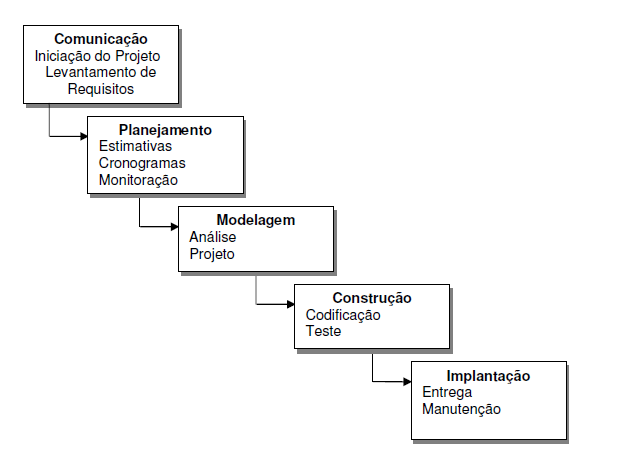
\includegraphics[width=10cm]{figuras/figura_ciclo_cascata}
\label{figura_ciclo_cascata}
\fnote{Fonte: \citeonline{pressman2006engenharia}}
\end{figure}

Dividimos o processo em nove atividades. A seguir, descreveremos brevemente cada uma delas:
\begin{enumerate}
	\item Iniciar Projeto: nessa atividade identificamos os objetivos do projeto, suas restri\c{c}\~oes, envolvidos, a organiza\c{c}\~ao da equipe de desenvolvimento e por \'ultimo realizamos uma 
reuni\~ao de in\'icio do projeto.
	\item Requisitos: nessa atividade realizamos o levantamento e an\'alise dos requisitos, sua documenta\c{c}\~ao, verifica\c{c}\~ao e valida\c{c}\~ao, al\'em de um estudo para saber atrav\'es dos 
requisitos se o projeto \'e vi\'avel. 
	\item Projeto: nessa atividade desenvolvemos o projeto da arquitetura do sistema, o planejamento dos m\'odulos, o projeto da interface gr\'afica com o usu\'ario  e como ser\~ao persistidos as 
entidades do sistema.
	\item Implementação: nessa atividade escolhemos primeiramente um m\'odulo do sistema para implementar, em seguida planejamos como ocorrer\'a a implementa\c{c}\~ao desse 
m\'odulo, implementamos o m\'odulo, e por \'ultimo realizamos a integra\c{c}\~ao de m\'odulo ao resto do sistema. Esse ciclo \'e repetido at\'e que todos os m\'odulos estejam desenvolvidos.
	\item Testes: durante essa atividade realizaremos o planejamento dos testes para o sistema, em seguida executaremos os testes para cada m\'odulo do sistema e para o sistema como um todo, e 
por \'ultimo iremos gerar um relat\'orio com os resultados dos testes.
	\item Implantação: ap\'os o sistema desenvolvido e devidamente testado, ele segue para a implanta\c{c}\~ao, em que prepararemos o ambiente onde o sistema ser\'a executado e realizaremos a 
implanta\c{c}\~ao. Ap\'os a implanta\c{c}\~ao, realizaremos testes de aceita\c{c}\~ao e a cria\c{c}\~ao de um manual para o sistema.
	\item Gerenciamento do Projeto: essa atividade ocorre durante todo o desenvolvimento do sistema e tem por objetivo permitir que o projeto consiga ser conclu\'ido dentro do prazo e da qualidade 
desejada.
	\item Avalia\c{c}\~ao do Processo: essa atividade \'e executada durante todo o desenvolvimento do projeto e permite que o processo utilizado seja constantemente avaliado e adaptado conforme segue 
o desenvolvimento do projeto.
	\item Encerrar Projeto: nessa \'ultima atividade ser\'a realizado apenas uma reuni\~ao em que ser\'a oficializado o final do projeto.
\end{enumerate}

O processo desenvolvido est\'a dispon\'ivel em \url{www.askmath.quixada.ufc.br/static/process/}. 

\subsection{Levantamento e Análise de Requisitos}


O Levantamento e An\'alise de Requisitos é a fase do desenvolvimento de um software em que o analista verifica junto ao usuário, quais as necessidades, condições e princípios que o \textit{software} 
deverá atender \cite{matuda2013mapas}. Essa fase possibilitou conhecer e estudar as necessidades do cliente, assim como as restrições que o software estará sujeito.

Para realizar a coleta dos requisitos, optamos por utilizar entrevistas com o cliente. Nessas entrevistas, que se caracterizarão como semi-estruturadas, já que foram guiadas por um roteiro previamente 
elaborado, composto por questões abertas \cite{belei2008uso}, foi possível obter os requisitos do sistema, assim como o público-alvo a quem o sistema atenderá. Essa técnica foi utilizada porque 
permitia uma organização flexível e ampliação dos questionamentos à medida que as informações foram sendo fornecidas pelo cliente \cite{fujisawa2000utilizaccao}.

O ambiente atender\'a quatro tipos de usu\'arios que formaram seu p\'ublico-alvo, ser\~ao administradores, professores, assistentes, e estudantes. Os administradores ser\~ao respons\'aveis por 
cadastrar 
novos professores, assim como realizar a manuten\c{c}\~ao di\'aria do sistema. Os professores ser\~ao responsáveis por definir as disciplinas e li\c{c}\~oes que faram parte do sistema. 
Ap\'os as disciplinas e li\c{c}\~oes definidas pelos professores, os assistentes ser\~ao respons\'aveis por manter os problemas de cada li\c{c}\~ao. Os estudantes resolver\~ao os problemas 
desenvolvidos pelos assistentes e poder\~ao postar d\'uvidas sobre qualquer conte\'udo no f\'orum de discuss\~oes. Quando o ambiente for aplicado em sala de aula, os professores ser\~ao ainda 
respons\'aveis por gerenciar suas turmas e acompanhar o andamento do progresso de cada um de seus estudantes, j\'a os assistentes ser\~ao responsáveis por tirar d\'uvidas dos estudantes no f\'orum 
de discuss\~oes.

Para uma melhor compreensão do público-alvo, foram criadas Personas 
\cite{pruitt2003personas}, personagens fictícios usados para caracterizar os papéis dos diferentes usuários do sistema \cite{guerra2010colaboraccao}. Cada persona criada possui um nome, hábitos, 
histórias pessoais, motivações, objetivos, entre outras (ver \nameref{apendice_personas}). A escolha dessa técnica deu-se pelo fato de que ela permitia ao desenvolvedor saber mais precisamente para 
quem ele deveria construir o sistema, além de permitir uma distinção maior do público-alvo e, dessa forma, aprofundar-se nos interesses individuais de cada um.

Apresentaremos a seguir, os principais requisitos levantados durante essa etapa:

\begin{alineascomponto}
	\item Hierarquia dos Conteúdos: no sistema, dever\~ao existir disciplinas, cada disciplina dever\'a possuir li\c{c}\~oes e cada li\c{c}\~ao ser\'a formada por problemas. Os professores poder\~ao 
cadastrar v\'arias disciplinas e li\c{c}\~oes, j\'a os assistentes ficar\~ao responsáveis por adicionar os problemas nas li\c{c}\~oes. Quando o estudante entrar no sistema, ele poder\'a ver somente 
as li\c{c}\~oes de uma disciplina por vez, podendo alternar entre disciplinas. Para um estudante come\c{c}ar a responder os problemas, ele dever\'a escolher inicialmente a disciplina e em seguida a 
li\c{c}\~ao. 

	\item Estrutura do Problema: cada problema possuir\'a uma descri\c{c}\~ao e v\'arios itens. Os problemas ser\~ao somente de m\'ultipla escolha e poder\~ao possuir no m\'inimo dois e no m\'aximo 
cinco itens, essa quantidade ficar\'a a crit\'erio do assistente que realizar\'a a adi\c{c}\~ao do problema no sistema.

	\item Saltar Problemas: o sistema deverá permitir ao aluno saltar problemas e rever os saltos 
realizados com algumas restrições na quantidade de saltos..
	
	\item Pedir Ajuda: para todo problema, o estudante poderá possuir uma ajuda. No momento em que o assistente estiver adicionando o problema, ele poderá ou não adicionar um texto de ajuda para o 
estudante, isso fica a critério dele. Quando o estudante estiver resolvendo os problemas, ele terá um botão que quando acionado, mostrar\'a o texto de ajuda. O sistema dever\'a salvar a quantidade 
de vezes que o estudante pedir ajuda e em quais problemas.
	
	\item Defici\^encias: \'e possível, a partir de um item respondido incorretamente em um problema, identificar a deficiência do estudante, por isso é fundamental que no momento que o 
assistente estiver adicionando os itens do problema, ele possa escolher para cada item incorreto, uma ou várias li\c{c}\~oes, essas lições ficarão sendo as supostas deficiências do aluno caso ele 
responda incorretamente aquele problema marcando aquele determinado item.
	
	\item F\'orum: o sistema deverá possuir um fórum onde os estudantes possam postar suas dúvidas para que professores, assistentes e outro participantes possam lhes ajudar com o problema. Esse fórum, deve possuir tópicos, comentários para os tópicos, e os comentários devem oferecer a opção de se comentar com imagens. 

\end{alineascomponto}

Após o levantamento dos requisitos, foi realizada a análise dos mesmos. Nessa análise, os requisitos foram agrupados em categorias. As categorias utilizadas são descritas por 
\citeonline{sommerville2003engenharia} como:
\begin{alineascomponto}
    \item Requisitos Funcionais -- especificam ações que um sistema deve ser
capaz de executar, sem levar em consideração restrições físicas. Os requisitos
funcionais especificam, portanto, o comportamento de entrada e saída de um
sistema.
    \item Requisitos Não Funcionais -- descrevem apenas atributos do sistema ou
atributos do ambiente do sistema, como segurança, desempenho, usabilidade e
confiabilidade.
    \item Requisitos de Domínio -- são os requisitos do domínio da aplicação do sistema e que refletem características desse domínio.
\end{alineascomponto}

Após esse agrupamento, os requisitos funcionais foram representados em Casos de Uso \cite{jacobson92engenharia}. Um caso de uso identifica os agentes envolvidos em uma interação e especifica o tipo 
de interação utilizando anotações sugeridas pela Unified Modeling Language (UML) 
\citeonline{sommerville2003engenharia}. Em seguida, foi realizada a documentação dos requisitos (ver \nameref{apendice_requisitos}).

No final dessa etapa, ocorreu a Validação dos Requisitos junto ao cliente.  A Validação dos Requisitos é definida como o processo que certifica que o modelo de requisitos gerado  esteja  consistente  
com  as  necessidades  e  intenções  de  clientes  e usuários \cite{rilston2003metodologia}. Esta etapa permitiu que os requisitos coletados e documentados estivesse de acordo com o que o 
cliente solicitou.

\subsection{Projeto do Sistema}

O Projeto de Software é à atividade de engenharia cujo foco é definir ``como'' os requisitos estabelecidos do projeto devem ser implementados no software \cite{pressman2006engenharia}. O objetivo da  atividade de projetar é gerar um modelo ou representação que apresente solidez, comodidade e deleite \cite{pressman2006engenharia}. 

Nesta fase, definimos como será aplicado o conhecimento obtido na pesquisa bibliográfica para se desenvolver o sistema. Para isto, definimos a arquitetura de software e as ferramentas que serão utilizadas durante o desenvolvimento do sistema. Nas seções a seguir, descrevemos um pouco sob cada um.

\subsubsection{Arquitetura}
Por arquitetura de software, entende-se a estrutura ou a organização de componentes de módulos, a maneira através da qual esses componentes interagem e a estrutura de dados que será usada pelos componentes \cite{pressman2006engenharia}.

A arquitetura utilizada baseia-se na arquitetura Cliente-Servidor\cite{david2013everything}, em que o processamento é dividido em processos distintos. Um processo é responsável pela manutenção da 
informação (servidor) e os outros são responsáveis pela captação de dados (clientes). Nessa arquitetura, os clientes enviam pedidos para o servidor, e este por sua vez processa estes dados e envia as 
respostas dos pedidos aos clientes.

Este modelo de arquitetura facilitará na manutenção do sistema, tendo em vista que toda atualização só necessitará ser realizada no servidor e automaticamente a mesma se propagará para todos os clientes. Com todos os recursos centralizados no servidor, podemos também ter um maior ganho com segurança, já que podemos centralizar os nossos esforços para manter a segurança das informações em apenas um único ponto, além de possibilitar que apenas cliente credenciados possam acessar e/ou alterar essas informações. Uma das outras grandes vantagens que temos  ao utilizar esse modelo, é que a medida que a quantidade de clientes aumente, será possível suprir esses clientes sem necessitar realizar nenhuma modificação essencial.

Para uma visualização mais detalhada da arquitetura de software definida, visitar o  \nameref{apendice_arquitetura}.

\subsubsection{Ferramentas}

 A análise do sistema foi feita com o auxílio da ferramenta de criação de diagramas Astah \cite{astah2016}, a implementação com a linguagem Python \cite{vanrossum2010python}, com o sistema de gerenciamento de banco de dados PostgresSQl \cite{momjian2001postgresql} e a camada de aplicação através da utilização do framework Django \cite{django2016}. Assim como a utilização do módulo Rosseta \cite{rosetta2016} para permitir a internacionalização do sistema.
 
A seguir, apresentaremos a lista das ferramentas e das tecnologias utilizadas para o desenvolvimento do projeto:

\begin{alineas}
	\item Astah: para a modelagem baseada em UML (Unified Modeling Language) do sistema.
	\item Python: linguagem de programação para implementação do sistema.
    \item Django: framework web responsável pela camada de aplicação.
    \item Rosetta: aplicação desenvolvida em Django que facilitará a tradução do projeto para diversas línguas.  
    \item PostgreSQL: como banco de dados para armazenamento e consulta de informações.
    \item Metro UI CSS: framework que faz uso de HTML, Cascading Stype Sheet (CSS) e Javascript para criação do front-end do sistema.
    \item MathJax: \'e uma engine\footnote{Uma biblioteca ou pacote de funcionalidades que são utilizadas para facilitar o desenvolvimento de alguma tecnologia.} de código aberto desenvolvido em 
javascript na forma de um plugin para incluir equações matemáticas em todos os navegadores, esse plugin aceita expressões em  MathML e Latex.

\end{alineas}

Essas ferramentas foram selecionadas por se tratarem, algumas, de ferramentas Open Source, ou seja, que seu código-fonte fonte pode ser alterado para diferentes fins, possibilitando assim que qualquer um consulte, examine ou as modifique, e outras por serem ferramentas que possibilitam um rápido desenvolvimento.

No final dessa etapa, foi gerado o Plano de Projeto, esse documento guiar\'a o desenvolvedor durante 
todo o processo de desenvolvimento.

\subsection{Implementação do Sistema}

A implementação envolve as atividades de codificação, compilação e integração. A codificação visa traduzir o design num programa, utilizando linguagens e  ferramentas adequadas. A codificação deve 
refletir a estrutura e o comportamento descrito no projeto. Os componentes arquiteturais devem ser codificados de forma independente e depois integrados \cite{aguiar2012requisitos}.

\subsection{Verificação e Validação}
Essa etapa destina-se a mostrar que o sistema está de acordo com a especificação 
e que ele atende às expectativas de clientes e usuários,  al\'em de assegurar 
que o  programa está fazendo aquilo que foi definido na sua especificação e que não 
possui  erros  de  execução \cite{aguiar2012requisitos}. 

Durante essa fase, ser\~ao realizados Testes de Unidade e Integra\c{c}\~ao em 
cada modulo do sistema, assim como Testes de Sistema no sistema j\'a integrado.

\citeonline{aniche2014teste} define essas categorias de Testes de Software como:

\begin{alineascomponto}
	\item Teste de Unidade -- é aquele que testa uma única unidade do sistema. 
Ele a testa de maneira isolada, geralmente simulando as prováveis dependências 
que aquela unidade tem. Em sistemas orientados a objetos, é comum que a unidade 
seja uma classe. Ou seja, quando queremos escrever testes de unidade para a 
classe Pedido, essa bateria de testes testará o funcionamento da classe Pedido, 
isolada, sem interações com outras classes.

	\item  Teste de Integração -- é aquele que testa a integração entre duas 
partes do seu sistema. Os testes que você escreve para a sua classe PedidoDao, 
por exemplo, em que seu teste vai até o banco de dados, é um teste de integração. 
Afinal, você está testando a integração do seu sistema com o sistema externo, 
que é o banco de dados. Testes que garantem que suas classes comunicam-se bem 
com serviços web, escrevem arquivos texto, ou mesmo mandam mensagens via socket 
são considerados testes de integração.

	\item Teste de Sistema -- \'e aquele que garante que o sistema funciona como um todo. Este 
nível de teste está interessado se o sistema funciona como um todo, com todas as 
unidades trabalhando juntas. Ele é comumente chamado de teste de caixa preta, já 
que durante o teste n\~ao se importa com a forma que os dados s\~ao processados, mas sim se as sa\'idas est\~ao de acordo com o que era esperado para entradas. 
\end{alineascomponto}

\subsection{Definição dos Conteúdo para o Sistema}

Após o sistema estar verificado e validado, ele terá que possuir conteúdos para ser utilizado pelo usuário final durante a fase de aplicação. A aplicação da primeira versão do sistema está planejada 
para ocorrer com uma turma de matemática da Universidade Federal do Ceará - Campus Quixadá. Decidimos optar por deixar os monitores\footnote{É o aluno de graduação concursado para exercer, juntamente 
com o professor, atividades técnico-didáticas condizentes com o seu grau de conhecimento junto à determinada disciplina, já por ele cursada.} da disciplina desenvolverem os conteúdos que ser\~ao 
utilizados no sistema durante essa fase. 

Os monitores passar\~ao por um treinamento, ao qual aprender\~ao a utilizar o sistema para, assim, adicionar os conteúdos desenvolvidos.

\subsection{Aplicação da Solução na Universidade Federal do Ceará - Campus Quixadá}

Aplicaremos o ambiente desenvolvido em duas turmas de Matemática Básica da UFC - Campus Quixadá. Nessas turmas, que est\'a previsto que sejam formadas por aproximadamente trinta estudantes 
cada, dividiremos os estudantes de cada turma em dois grupos, Grupo A1 e Grupo B1 para a primeira turma e Grupo A2 e B2 para a segunda turma. Os Grupos A1 e A2, ser\~ao formados pela metade 
dos estudantes de cada turma, escolhidos aleatoriamente, e os Grupos B1 e B2 pelos estudantes restantes. 
Esta divisão, deve-se ao fato de que ao final da experiência de utilização do ambiente pelos estudantes, realizaremos uma comparação no desempenho entre estudantes que utilizaram o sistema com os que 
não utilizaram. Dessa forma, o sistema será utilizado pelos estudantes dos Grupos A1 e A2, enquanto que os Grupos B1 e B2 (grupos de controle) continuaram estudando da mesma forma. 

O objetivo dessa experiência e analisar o impacto que o uso do ambiente desenvolvido tem na aprendizagem dos estudantes. Os dados que iremos utilizar para atingirmos os objetivos com essa 
experiência ser\~ao providos de duas avalia\c{c}\~oes realizadas por todos os alunos das duas turmas antes e depois a utiliza\c{c}\~ao do ambiente pelos Grupos A1 e A2.

\subsection{Cronograma de Execução}
\begin{table}[H]
\centering
\caption{Cronograma de Execução}
\label{cronograma}

\resizebox{\textwidth}{!}{
\begin{tabular}{|l|c|c|c|c|c|c|c|c|c|c|c|c|c|c|c|}
\hline
\multicolumn{1}{|c|}{\multirow{2}{*}{ATIVIDADES}} & \multicolumn{6}{c|}{2015} & \multicolumn{9}{c|}{2016} \\ \cline{2-16} 
\multicolumn{1}{|c|}{} & Jan & Fev & Mar & Abr & Mai & Jun - Dez & \multicolumn{1}{l|}{Jan - Mar} & \multicolumn{1}{l|}{Abr} & \multicolumn{1}{l|}{Mai} & \multicolumn{1}{l|}{Jun} & \multicolumn{1}{l|}{Jul} & \multicolumn{1}{l|}{Ago} & \multicolumn{1}{l|}{Set} & \multicolumn{1}{l|}{Out} & \multicolumn{1}{l|}{Nov} \\ \hline
Definição do Processo & x &  &  &  &  &  &  &  &  &  &  &  &  &  &  \\ \hline
Levantamento e Análise dos Requisitos & x & x & x &  &  &  &  &  &  &  &  &  &  &  &  \\ \hline
Projeto do Sistema &  &  &  & x & x &  &  &  &  &  &  &  &  &  &  \\ \hline
Implementação do Sistema &  &  &  &  &  & x & x & x & x & x &  &  &  &  &  \\ \hline
Verificação e Validação &  &  &  &  &  &  &  &  &  &  & x &  &  &  &  \\ \hline
Desenvolver o conteúdo para o sistema &  &  &  &  &  &  &  & x & x & x & x & x &  &  &  \\ \hline
Aplicação na UFC - Campus Quixadá &  &  &  &  &  &  &  &  &  &  &  & x & x & x &  \\ \hline
Definição do Projeto de Pesquisa &  &  &  &  &  &  &  & x &  &  &  &  &  &  &  \\ \hline
Defesa do Projeto de Pesquisa &  &  &  &  &  &  &  &  &  & x &  &  &  &  &  \\ \hline
Ajustes Solicitados &  &  &  &  &  &  &  &  &  &  & x &  &  &  &  \\ \hline
Análise dos Resultados Obtidos na Aplicação. &  &  &  &  &  &  &  &  &  &  &  &  &  &  & x \\ \hline
Defesa do Trabalho Final &  &  &  &  &  &  &  &  &  &  &  &  &  &  & x \\ \hline
\end{tabular}}
\fnote{Fonte: Elaborado pelo autor}
\end{table}


\section{RESULTADOS PRELIMINARES}

Nesta seção apresentaremos o andamento deste trabalho.

Até o momento, de concluído, temos o processo que está sendo utilizado durante o desenvolvimento do sistema, os requisitos do sistema que já foram coletados, analisados e validados, além do próprio projeto do sistema. 

Na fase que está em andamento, que é a fase de implementação, temos os seguintes módulos concluídos: 

\begin{alineascomponto}
	\item Gerenciador de Usuários: módulo responsável por gerenciar os usuários do sistema como professores, assistentes e alunos.
	\item Gerenciador de Turmas: módulo responsável por gerenciar as turmas de alunos do sistema.
    \item Gerenciador de Disciplinas: módulo responsável por gerenciar as disciplinas que serão cadastradas no sistema.
    \item Gerenciador de Lições: módulo responsável por gerenciar as lições que os professores irão cadastrar no sistema.
    \item Gerenciador de Questões: módulo responsável por gerenciar os problemas que os assistentes e professores poderão cadastrar para cada lição.
    \item Gerenciador de Pontuação: módulo responsável por gerenciar a pontuação ganha pelos alunos, assim como seu nível de experiência ao longo da utilização do sistema. 
    \item Fórum: módulo responsável por permitir que alunos postem dúvidas dos mais variados  assuntos relacionadas ao sistema, seja dúvidas em relação ao conteúdo apresentado em sala de aula, assim como informações sobre o sistema e sugestões. 
\end{alineascomponto}

Os módulos que ainda restam para serem desenvolvidos nesta fase são:

\begin{alineascomponto}
	\item Gerenciador de Progresso: módulo responsável por acompanhar o andamento de cada estudante durante seu aprendizado e identificar os obstáculo epistemológicos enfrentados, indicando ao aluno 
a exist\^encia desses obst\'aculos e o(s) conte\'udo(s) que ele possui defici\^encia (causador(es) do obstáculo) para ele assim poder pausar o conte\'udo que est\'a estudando e voltar a 
estudar o(s) conte\'udo(s) que o sistema indicar.

	\item Gerador de Estatísticas: módulo responsável por gerar as estatísticas que o professor utilizará para acompanhar o andamento de suas turmas e alunos, assim como para o uso pelo estudante, 
que utilizará para acompanhar seu próprio progresso durante sua aprendizagem no sistema.
    
    \item Ranking: módulo responsável por manter um ranking\footnote{É uma classificação ordenada de acordo com critérios determinados.} com os posicionamentos dos alunos de acordo com seu desempenho 
no sistema durante a semana.
    
\end{alineascomponto}

A seguir, apresentaremos algumas telas do sistema:

\begin{figure}[H]
  \centering
  \begin{minipage}[b]{0.49\textwidth}
	\caption{Tela Inicial}
    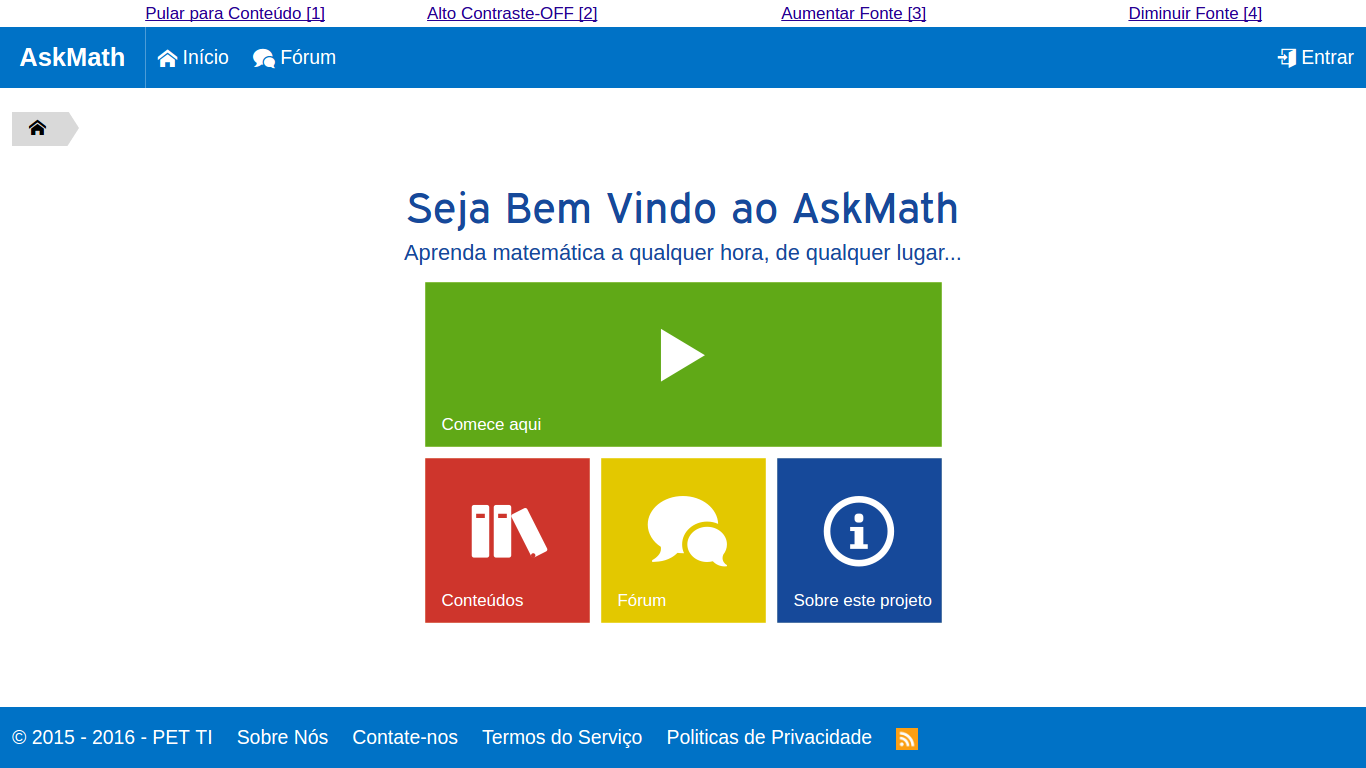
\includegraphics[width=\textwidth]{figuras/askmath/1}
    \fnote{Fonte: \url{www.askmath.quixada.ufc.br}.}
  \end{minipage}
  \hfill
  \begin{minipage}[b]{0.49\textwidth}
	\caption{Tela Inicial do Estudante}
    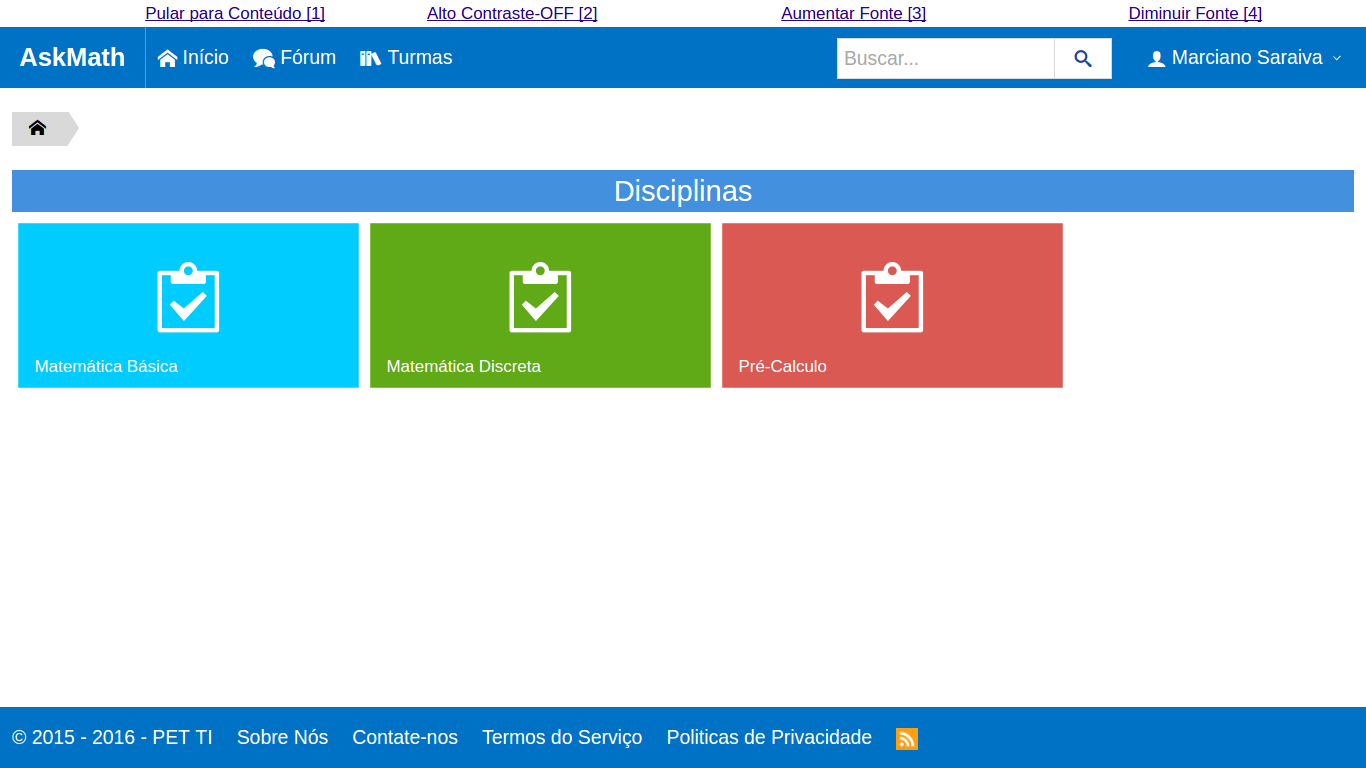
\includegraphics[width=\textwidth]{figuras/askmath/2}
  	\fnote{Fonte: \url{www.askmath.quixada.ufc.br}.}
  \end{minipage}
 
  \begin{minipage}[b]{0.49\textwidth}
    \caption{Tela de Administra\c{c}\~ao}
    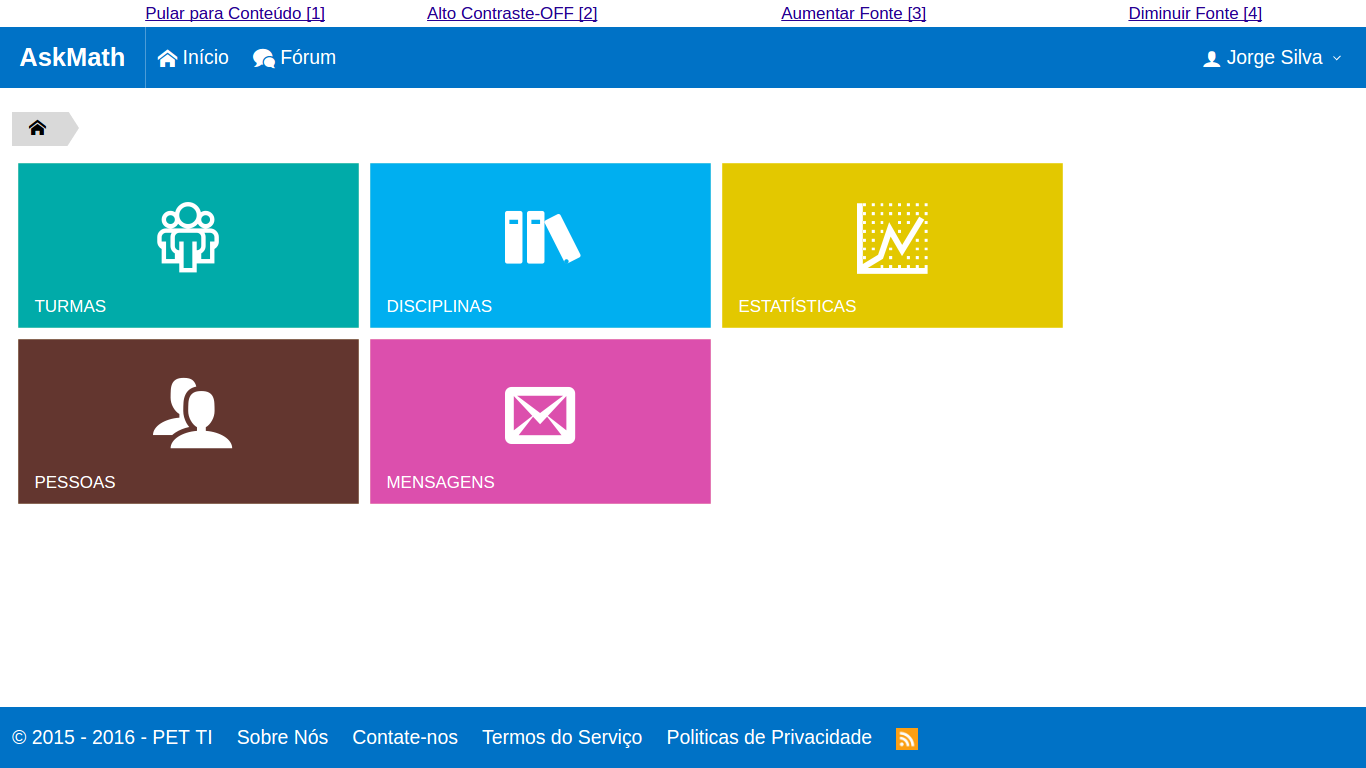
\includegraphics[width=\textwidth]{figuras/askmath/3}
    \fnote{Fonte: \url{www.askmath.quixada.ufc.br}.}
  \end{minipage}
  \hfill
  \begin{minipage}[b]{0.49\textwidth}
	\caption{Tela de Problemas do Estudante}
    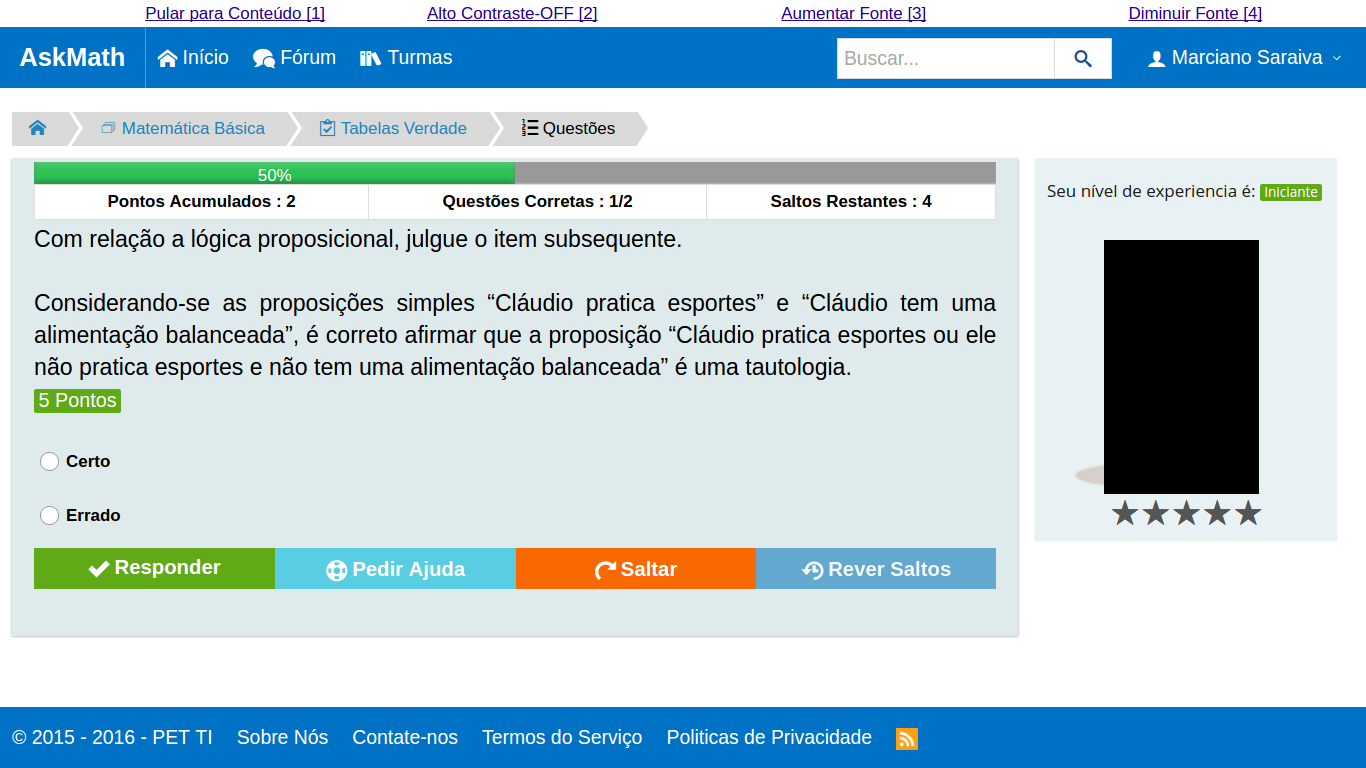
\includegraphics[width=\textwidth]{figuras/askmath/4}
    \fnote{Fonte: \url{www.askmath.quixada.ufc.br}.}
  \end{minipage}
\end{figure}

Os conteúdos que serão utilizados para popular o sistema, durante sua aplicação na UFC-Campus Quixadá, já estão sendo desenvolvidos pelos monitores citados anteriormente. Após a validação e verificação do sistema, esses conteúdos serão adicionados por esses monitores, que passaram por um treinamento para aprenderem a utilizar o sistema.









\newpage

% ----------------------------------------------------------
% ELEMENTOS PÓS-TEXTUAIS
% ----------------------------------------------------------
%\postextual

% Referências bibliográficas

\bibliography{bibtex/referencias}
\addcontentsline{toc}{chapter}{REFERÊNCIAS}

\newpage

% Glossário (Consulte o manual da classe abntex2 para orientações sobre o glossário)
%\glossary

% Apêndices
% Apêndices
% ---
% Inicia os apêndices
% ---
\begin{apendicesenv}

% Imprime uma página indicando o início dos apêndices
\partapendices

% ----------------------------------------------------------
\chapter{Quisque libero justo}
% ----------------------------------------------------------

\lipsum[50]

% ----------------------------------------------------------
\chapter{Nullam elementum urna vel imperdiet sodales elit ipsum pharetra ligula
ac pretium ante justo a nulla curabitur tristique arcu eu metus}
% ----------------------------------------------------------
\lipsum[55-57]

\end{apendicesenv}
% ---


% Anexos
% % ----------------------------------------------------------
% Anexos
% ---
% Inicia os anexos
% ---

\apendice{ANEXO A}
\addcontentsline{toc}{section}{ANEXO A}

Contém documentos de outros autores, quando aplicável. Se não for utilizada, esta seção deve ser removida já na versão 1 do projeto.

%---------------------------------------------------------------------
% INDICE REMISSIVO
%---------------------------------------------------------------------
%\phantompart
%\printindex
%---------------------------------------------------------------------

\end{document}